\documentclass{jarticle}

% 余白の設定
\usepackage[top=30truemm, bottom=30truemm, left=25truemm, right=25truemm]{geometry}

% タイトルの文字サイズを本文に合わせる
\usepackage{titlesec}
\titleformat*{\section}{\normalsize}
\titleformat*{\subsection}{\normalsize}

% 画像の描画
\usepackage[dvipdfmx]{graphicx}

% 図, 表, 式番号のつけ方
% TODO 図表式番号を一括で振る
\makeatletter
  \def\thefigure{\thesection.\arabic{figure}}
  \@addtoreset{figure}{section}
  \renewcommand{\thetable}{\arabic{section}.\arabic{table}}
  \renewcommand{\theequation}{\arabic{section}.\arabic{equation}}
  \@addtoreset{table}{section}
  \@addtoreset{equation}{section}
\makeatother

% プログラムリスト
\usepackage{listings}
\lstset{basicstyle=\ttfamily\footnotesize,frame=single}


\begin{document}

\begin{center}
  タイトル
\end{center}

\begin{flushright}
  出題日:\\
  提出日:\\
  学籍番号:\\
  所属 学年 名前
\end{flushright}

\section{セクションタイトル}

\subsection{サブセクションタイトル}

ここに本文を書いていく.

\section{各種オブジェクトの挿入}

\subsection{図の挿入}

図を挿入したらlabelで図番号を参照できる.
図\ref{chart1}みたいな感じ.

\begin{figure}[htb]
  \begin{center}
    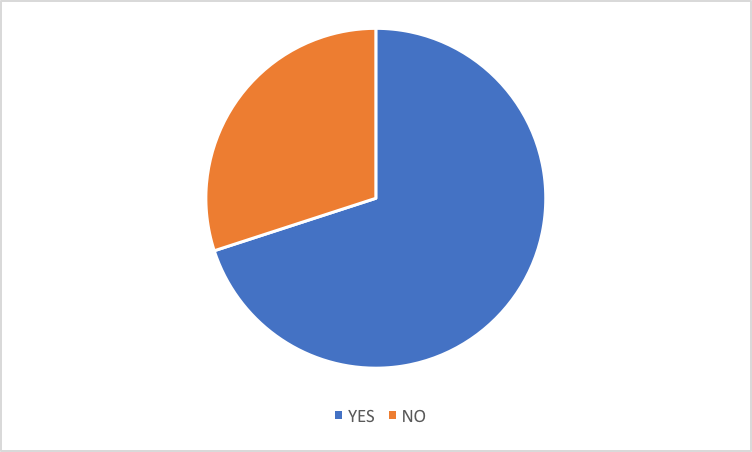
\includegraphics[keepaspectratio, scale=1.0]{chart1.png}
    \caption{キャプション}
    \label{chart1}
  \end{center}
\end{figure}

\subsection{表の挿入}

表を挿入したらlabelで表番号を参照できる.
表\ref{table1}みたいな感じ.

\begin{table}[htb]
  \begin{center}
    \caption{キャプション}
    \label{table1}
    \begin{tabular}{c|c|c}
      \hline
      1 & 2 & 2 \\
      \hline \hline
      AAA & CCCCC & EEEEE \\
      BBB & DDDDD & FFFFF \\
      \hline
    \end{tabular}
  \end{center}
\end{table}

\subsection{プログラムの挿入}

プログラムを直接埋め込むことができる.

\begin{lstlisting}
#include <cstdio.h>

int main(void) {
  printf("Hello, World\n");
  return 0;
}
\end{lstlisting}

ファイルを指定してプログラムを埋め込むこともできる.

\lstinputlisting{program1.c}

\end{document}
